%Here is the method used to examine the question
In this chapter, the methods employed to answer the proposed question are presented. This chapter begins by establishing the task as well as the datasets and data processing utilized in this project. Thereafter, the experimental setup is described and relevant neural network architectures are outlined. Finally, the approaches for training the generative models are presented. Three approaches of this kind have been employed in this project: standard \acrfull{vaes}, progressive \acrfull{gans} and Autoencoding \acrfull{gans}. They are presented in their respective section. 

The level of detail presented here should suffice for re-implementing the algorithms and repeat the experiments of this project. There certainly exist questions which need more details to answer than what can possibly be captured in a report like this. For further details that allows replicating the experiments, the original implementation is available online\footnote{The code is available at: \url{www.github.com/netrome/DeepGeneration}}.

\section{Pupil Localization}
\begin{figure}[t]
    \centering
    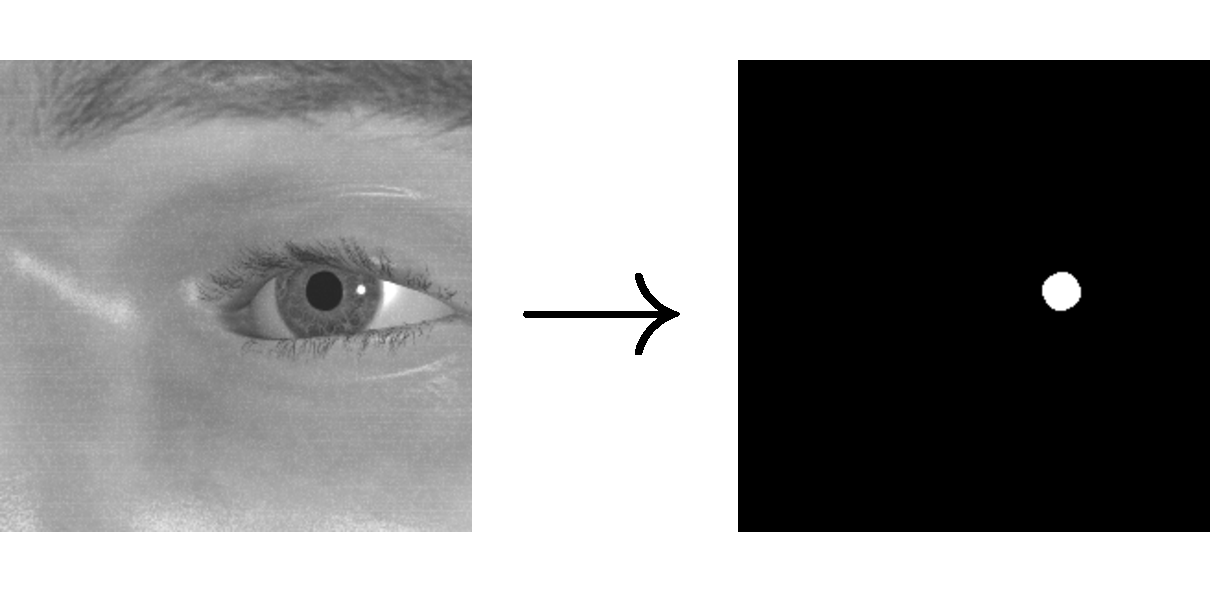
\includegraphics[width=\textwidth]{images/misc/pupil-localization.pdf}
    \caption{Pupil localization is the problem of finding the position and shape of the pupil in an image of an eye, such as the one to the left in this figure. This problem can be represented as a semantic segmentation problem, wehre the goal is to learn a mapping between the image and a segmentation map corresponding to the pupil in the image, positioned right of the image of the eye.}
    \label{fig:pupillocalization}
\end{figure}
To investigate the extent to which deep generative models can act as a drop-in replacement for real datasets, a case study of pupil localization was performed. Pupil localization is an instance of the object localization problem. The objective is to localize the pupil in an image of an eye. This problem can be formulated as a semantic segmentation problem as illustrated in figure \ref{fig:pupillocalization}. In normal cases, pupil localization is not achieved with deep neural networks. There already exist more computationally efficient methods for this task, such as the method proposed in \parencite{markuvs2014eye}. On the other hand, deep neural networks for semantic segmentation are capable of predicting high quality segmentation maps on diverse complicated datasets \parencite{ChenPK0Y16semantic} and should therefore perform extraordinary well on the relatively simple task of pupil localization.

By comparing pupil localization performance when the localizer is trained on either data from a deep generative model or data from the original dataset and tested on data from either of the domains, the usability of the generated data for model training or evaluation can be assessed. This becomes especially interesting in the case of training on generated data and testing on the original data. Assuming that the localizer learns the optimal mapping for the data domain it is trained on, the performance of this localizer can then be used as a measure of the quality and usability of the generated data. 

The benefit of this approach is that the relative magnitudes of the errors obtained when training on one dataset and testing on another indicate the difficulties of adapting models between these domains. This does not only give a binary answer to the original question of this project but also shows how close the tested methods are to learning the data distribution. %\todocomment{Good summary of the point}

%The benefit of this approach is that the cross-data localization error can easily be compared to the intra-data localization error. The relative magnitutes of these losses indicate the difficulties of adapting models between the domains. This enables not only giving a binary answer to the original question of this project but showing how close to succeeding the tested methods are in learning the data distribution.

\section{Synthetic Data}
\begin{figure}[t]
    \centering
    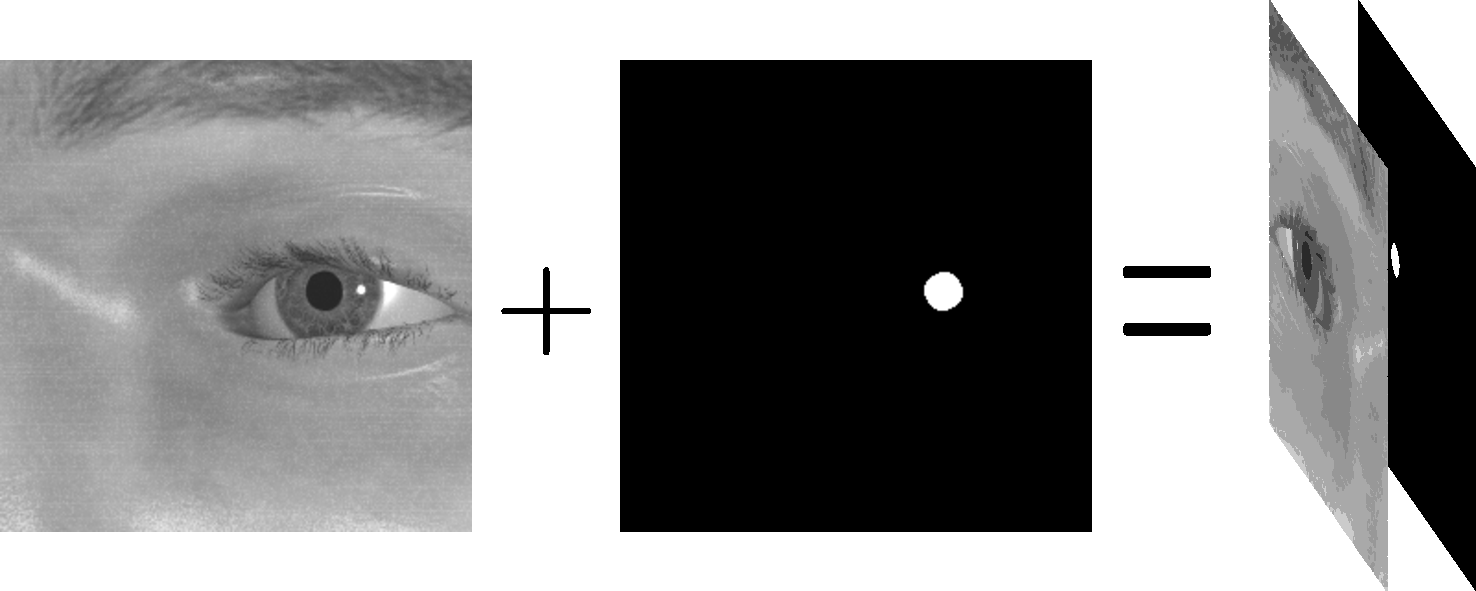
\includegraphics[width=\textwidth]{images/misc/2-channel_img_example2.pdf}
    \caption{Example of how a $256\times256$ image can be concatenated together with a segmentation map to form a single 2-channel image. The segmentation map in this case corresponds to the pupil in the image.}
    \label{fig:2channels}
\end{figure}

The initial experiments in this project are performed on synthetic data obtained through the rendering of a 3D head model in a data generation framework. This framework is based on the work of \textcite{swirski2014rendering} and utilizes the same head rig. Two datasets with resolution $256\times256$ were generated, a training set consisting of $3000$ images and a test set of $300$ images. For reproducibility, these datasets are publicly available\footnote{The datasets are hosted at: \url{www.kaggle.com/netrome/deepgenerationsynthetic}}.

The synthetic datasets are fully annotated with automatically generated ground truth labels. The relevant labels for the experiments are converted to heatmaps when loaded for training and evaluation as in most cases of semantic segmentation \parencite{guo2017review}. These heatmaps are thereafter concatenated with the real images, forming feature maps with the dimensions $2\times256\times256$. An example of this procedure is illustrated in figure \ref{fig:2channels}. By viewing the annotations as a part of the data, unsupervised models that learn the data distribution implicitly learn the relationships between the annotations and the images. Figure \ref{fig:2channelsGAN} and \ref{fig:2channelsVAE} show how this type of data is processed in a \acrshort{vae} and a \acrshort{gan}.

\begin{figure}[t]
    \centering
    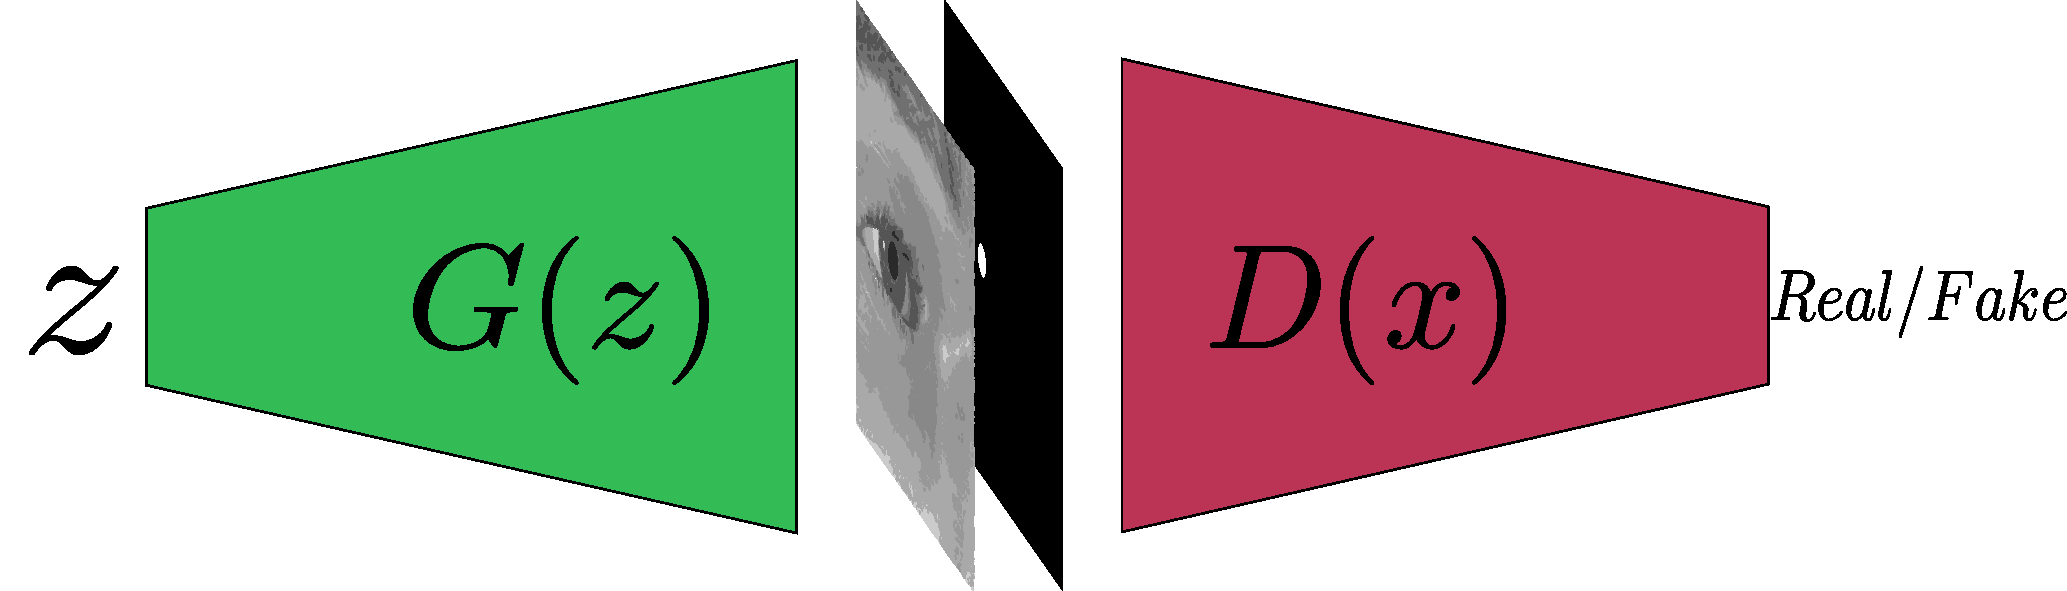
\includegraphics[width=\textwidth]{images/misc/GAN_illustration_for_methods.pdf}
    \caption{Example of a \acrshort{gan} where the generator generates a 2-channel image and the discriminator distinguishes fake 2-channel images from real ones. The training procedure is the same as that of a normal \acrshort{gan}}
    \label{fig:2channelsGAN}
\end{figure}

\begin{figure}[t]
    \centering
    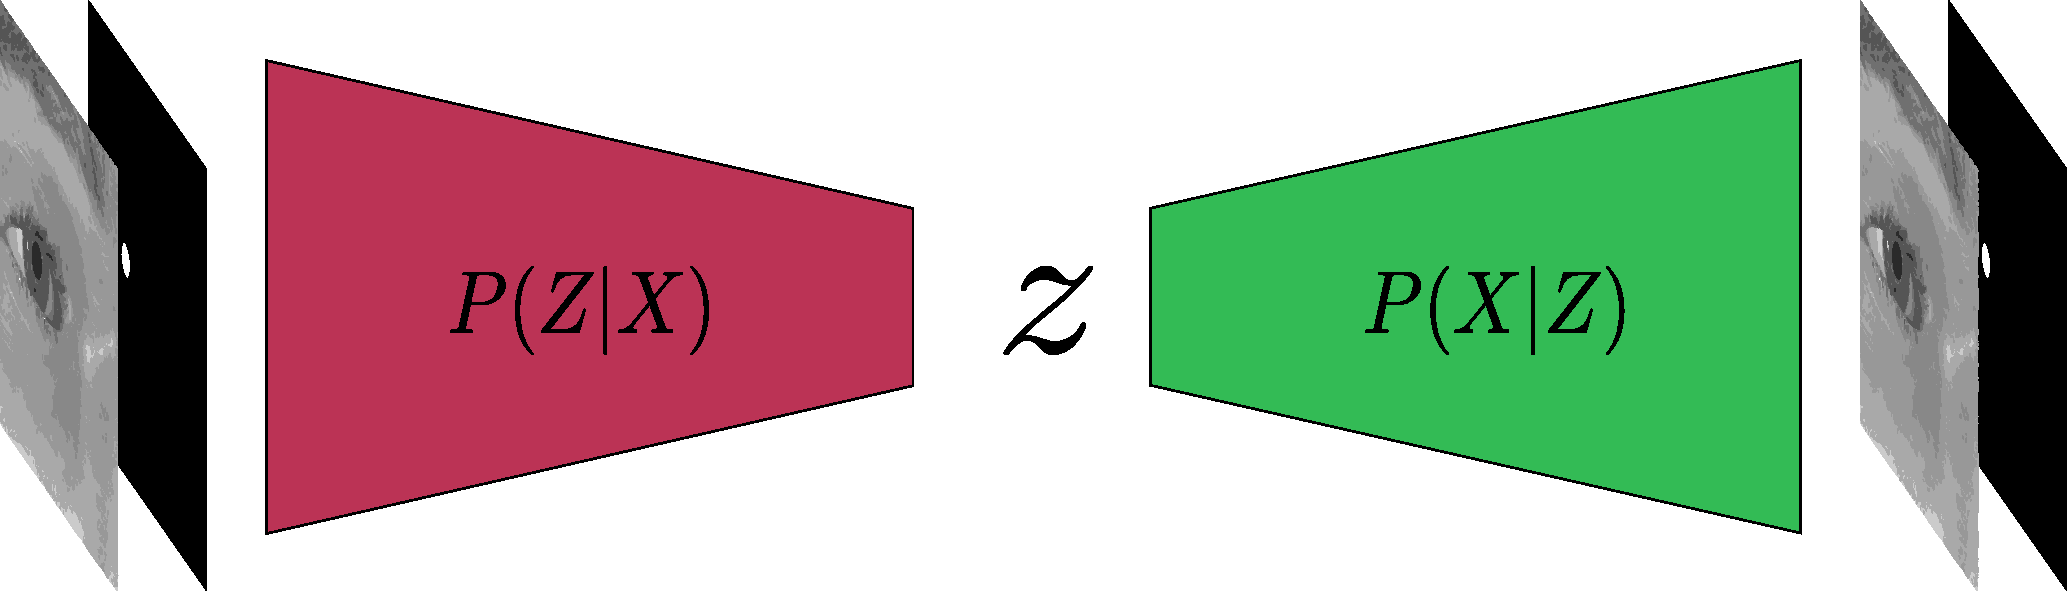
\includegraphics[width=\textwidth]{images/misc/VAE_illustration_for_methods.pdf}
    \caption{Example of a \acrshort{vae} where the encoder generates a probability distribution in the latent space conditioned on a 2-channel image and the decoder maps a latent vector to a conditional probability distribution over 2-channel images.}
    \label{fig:2channelsVAE}
\end{figure}


\section{Real World Data}
\begin{figure}[t]
    \centering
    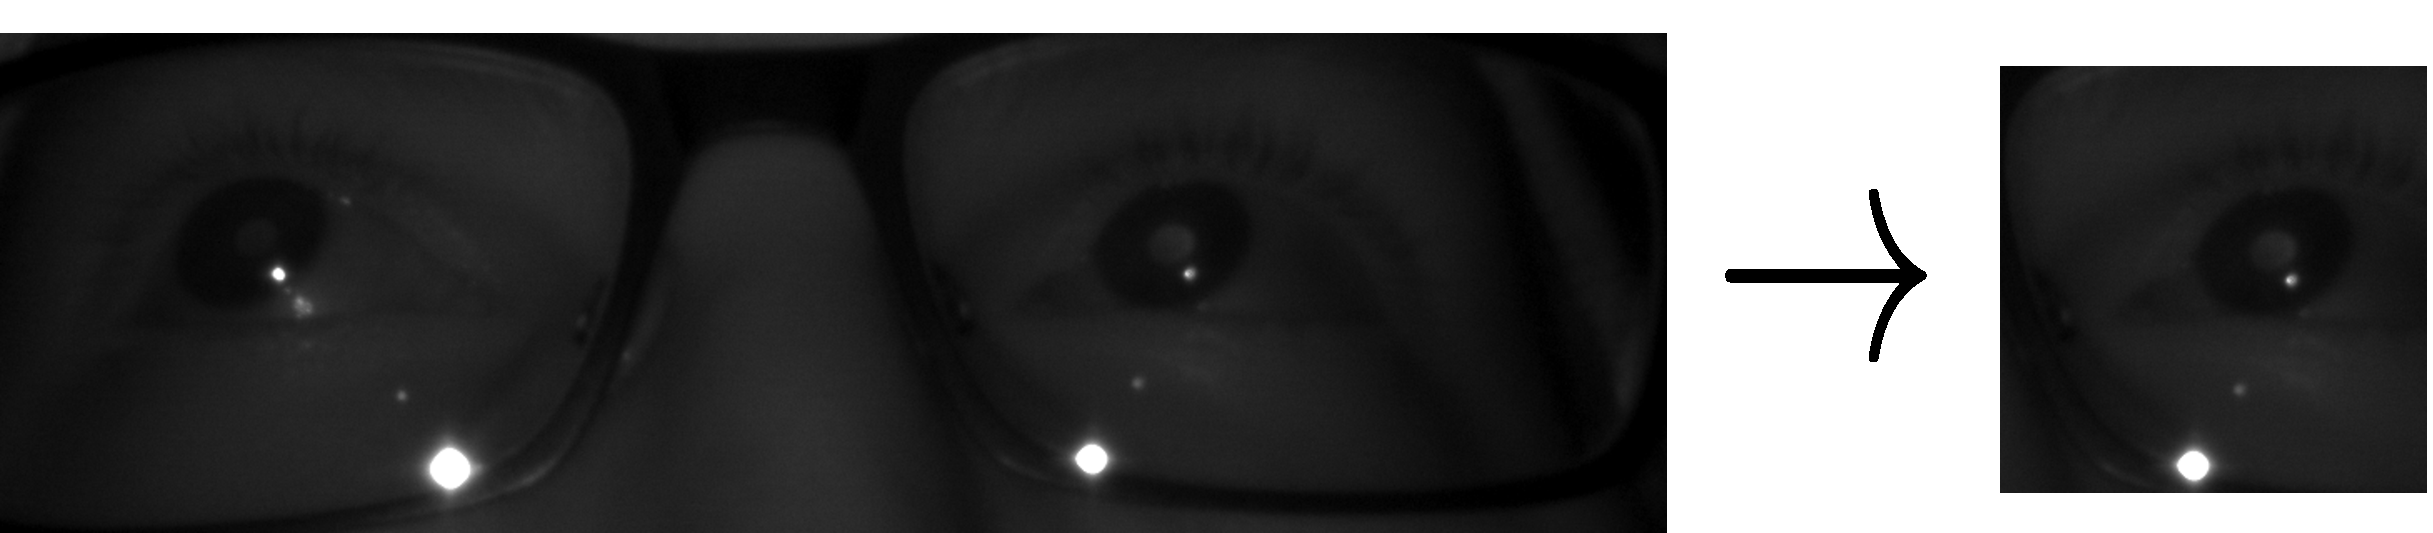
\includegraphics[width=\textwidth]{images/misc/roi_to_crop.pdf}
    \caption{A \acrshort{roi} image and a corresponding $256\times256$ crop of the right eye illustrating the processing of the real world data.}
    \label{fig:roitocrop}
\end{figure}
A propiretary dataset was used to further evaluate the methods. The dataset consists of $9605$ different manually annotated recordings of human subjects looking at a screen, split into a training set of $8605$ recordings and a test set of $1000$ recordings. Each recording consists of a set of \acrfull{roi} images of the eye region of the subjects. 

To adapt this data to the Pupil Regression framework, the images were cropped to $256\times256$ patches around the eyes. An example crop together with its corresponding \acrshort{roi} image is shown in figure \ref{fig:roitocrop}. The cropping was random and ensured that the images always contained a pupil. In practical cases it would be sensible to center the pupil in all images. For this purpose however, such a cropping would cause the networks to learn undesired patterns such as always producing trivial predictions in the center of the image. Therefore the center of the pupil was positioned randomly in the image during the cropping. 

During data sampling, the probabilites of the individual images were weighted in such a way that the separate recordings were equally probable to appear. This prevents recordings with more images to be over-represented during training, which otherwise could cause the models to become skewed to the conditions of these recordings.

\section{Network architectures}
The deep generative models as well as the Pupil localizer are based on deep convolutional neural networks. There are four different types of networks that are utilized in the different models in this work: generators, discriminators, encoders and transformers. These types describe the transformations the networks represent.

The default generator architecture is outlined in table \ref{tab:generator}. The default discriminator architecture is outlined in table \ref{tab:discriminator}. The main structure of these networks follows the architectures used by \textcite{karras2017progressive}, but the feature maps are smaller in this project and instead of using non-parametric upsampling followed by an extra convolution, the upsampling is performed with transposed convolutions. These changes are motivated by the limited time-frame of this project as they enable faster training of the networks. Furthermore, the datasets of this project are believed to be less complex than those of \textcite{karras2017progressive}, whereby less parameters should be necessary for the networks to capture the essence of the datasets.

The encoder follows the structure of the discriminator but does not use minibatch discrimination, and the output shape is adjusted to the size of the latent space instead of producing a scalar output. 

The transformer is only used for Pupil Localization and is an image-to-image network. The structure of the transformer is shown in table \ref{tab:transformer}. The main structure resembles that of \textcite{ronneberger2015u}, but many details are different. 
%\todocomment{is it worth discussing those differences?} - No /M

%...relevant network architectures are described here, together with figures and stuff. Base it around GAN networks, the small differences in the encoders can be explained afterwards.

\begin{table}[t]
    \centering
    \caption{Generator architecture used in the experiments. Feature normalization and leaky ReLUs were applied after each convolution except the last one. Note that input is not technically an operation but it can be viewed as an identity operation and is included here to illustrate the input shape in a concise manner.}
    \label{tab:generator}
    \begin{tabular}{|lll|}
        \hline
        %\multicolumn{3}{c}{Generator}           \\ 
        Operation          & Output shape     & Stride \\ \hline
        Input              & $128\times1\times1$   &$1$     \\
        Conv 4x4           & $128\times4\times4$   &$1$     \\
        Conv 3x3           & $128\times4\times4$   &$1$     \\ \hline
        Transpose Conv 2x2 & $128\times8\times8$   &$2$     \\
        Conv 3x3           & $112\times8\times8$   &$1$     \\ \hline
        Transpose Conv 2x2 & $112\times16\times16$   &$2$     \\
        Conv 3x3           & $96\times16\times16$   &$1$     \\ \hline
        Transpose Conv 2x2 & $96\times32\times32$   &$2$     \\
        Conv 3x3           & $80\times32\times32$   &$1$     \\ \hline
        Transpose Conv 2x2 & $80\times64\times64$   &$2$     \\
        Conv 3x3           & $64\times64\times64$   &$1$     \\ \hline
        Transpose Conv 2x2 & $64\times128\times128$   &$2$     \\
        Conv 3x3           & $32\times128\times128$   &$1$     \\ \hline
        Transpose Conv 2x2 & $32\times256\times256$   &$2$     \\
        Conv 3x3           & $16\times256\times256$   &$1$     \\ \hline
        Conv 1x1           & $2\times256\times256$ &$1$       \\ \hline
    \end{tabular}
\end{table}

\begin{table}[t]
    \centering
    \caption{Discriminator architecture, Leaky ReLUs were applied after each convolution except the last one. }
    \label{tab:discriminator}
    \begin{tabular}{|lll|}
        \hline
        %\multicolumn{3}{c}{Discriminator}           \\ 
        Operation          & Output shape     & Stride \\ \hline
        Input              & $2\times256\times256$   &$1$  \\
        Conv 1x1           & $16\times256\times256$ &$1$   \\ 
        Conv 3x3           & $32\times256\times256$ &$1$   \\ 
        Conv 2x2           & $32\times128\times128$ &$2$   \\ \hline
        Conv 3x3           & $64\times128\times128$ &$1$   \\ 
        Conv 2x2           & $64\times64\times64$ &$2$     \\ \hline
        Conv 3x3           & $80\times64\times64$ &$1$     \\ 
        Conv 2x2           & $80\times32\times32$ &$2$     \\ \hline
        Conv 3x3           & $96\times32\times32$ &$1$     \\ 
        Conv 2x2           & $96\times16\times16$ &$2$     \\ \hline
        Conv 3x3           & $112\times16\times16$ &$1$    \\ 
        Conv 2x2           & $112\times8\times8$ &$2$      \\ \hline
        Conv 3x3           & $128\times8\times8$ &$1$      \\ 
        Conv 2x2           & $128\times4\times4$ &$2$      \\ \hline
        Minibatch stddev
        Conv 3x3           & $128\times4\times4$   &$1$    \\
        Conv 4x4           & $128\times1\times1$   &$1$    \\ 
        Fully connected    & 1x1 &$1$        \\ \hline
    \end{tabular}
\end{table}

\begin{table}[t]
    \centering
    \caption{Transformer architecture used in the experiments. Skip layers were introduced as indicated in the table. Leaky ReLUs were applied after each convolution except the last one. In the prescence of skip connections the addition of the feature maps was performed before the Leaky ReLUs were applied.}
    \label{tab:transformer}
    \begin{tabular}{|lll|}
        \hline
        %\multicolumn{3}{c}{Generator}           \\ 
        Operation           & Output shape  & Stride \\ \hline
        Input               & $1\times256\times256$     &$1$    \\
        Conv 1x1 (1)           & $16\times256\times256$    &$1$    \\
        Conv 3x3 (2)            & $32\times128\times128$    &$2$    \\    
        Conv 3x3 (3)           & $64\times64\times64$    &$2$    \\ 
        Conv 3x3 (4)           & $128\times32\times32$    &$2$   \\ 
        Conv 3x3 (5)           & $256\times16\times16$    &$2$   \\ 
        Conv 3x3 (6)           & $256\times8\times8$     &$2$   \\ 
        Conv 3x3            & $256\times4\times4$    &$2$   \\ \hline
        Transpose Conv 4x4 + (6)  & $256\times8\times8$    &$2$   \\
        Transpose Conv 4x4 + (5) & $256\times16\times16$    &$2$   \\
        Transpose Conv 4x4 + (4) & $128\times32\times32$    &$2$   \\
        Transpose Conv 4x4 + (3) & $64\times64\times64$    &$2$   \\
        Transpose Conv 4x4 + (2) & $32\times128\times128$    &$2$   \\
        Transpose Conv 4x4 + (1)  & $16\times256\times256$    &$2$   \\
        Conv 1x1            & $1\times256\times256$    &$1$    \\ \hline
    \end{tabular}
\end{table}

\section{\acrlong{vaes}}
A \acrlong{vae} was constructed and trained on the synthetic data as a baseline for further experiments. The advantages of using \acrshort{vaes} for data generation in contrast to \acrshort{gans} are that they are easier to train and do not suffer from vanishing modes of data.

The \acrlong{vae} was designed using the default generator (the one from Table \ref{tab:generator}) network as a decoder and the default encoder network with an output shape of $128\times2$. In this framework, the encoder output is interpreted as the mean vector and the diagonal covariance matrix of a 128-dimensional Gaussian distribution. Using $Enc$ to denote the encoder function, this can be formulated as $P(Z|X=x) \sim \mathcal{N}(\mu, \sigma)$, where $(\mu, \sigma) = Enc(x)$. Furthermore, the posterior $P(X|Z=z)$ is modelled as a Laplace distribution where the mean value is the generator output as $P(X|Z=z) \sim \text{Laplace}(G(z), b)$, where $b$ is taken to be a hyperparameter. From a deep learning perspective this is equivalent to training the \acrshort{vae} with a $L_1$ reconstruction loss. The training objective can then be formulated as 
\begin{equation}
    L_{VAE}(\theta) = \lambda D_{KL}\left(P(Z|X=x) || \mathcal{N}(0,1)\right) + |\hat{X} - X|_1,
\end{equation}
where $\hat{X}$ is the reconstructed image, $D_{KL}$ is the Kullback-Leibler divergence \parencite{kullback1951information}, $\theta$ is the parameters used for modelling $P(Z|X)$ and $P(X|Z)$ and $\lambda$ is a scale parameter that controls the trade-off between the KL term and the reconstruction loss. Scaling the KL loss has the same relative effect between the two loss terms as adjusting the $b$ parameter in the Laplacian distribution, and fixing the weight of the $L_1$ loss instead of the KL-loss means that a sensible learning rate in this setting should be similar to that of a normal autoencoder. 

\section{\acrlong{wgan}}
The \acrfull{wgan} was adopted as a second baseline to compare against more complex methods. It was chosen because it currently is one of the most prominent \acrshort{gan} variations. Furthermore the progressive \acrshort{gan} is based on the \acrshort{wgan} causing the \acrshort{wgan} to be both a natural baseline for the evaluation and a special case of the progressive \acrshort{gan}. 

The \acrshort{wgan} was constructed using the default generator and discriminator. To enforce the discriminator to be 1-Lipschitz \footnote{The relevant theory of Lipschitz analysis is presented in \parencite{heinonen2005lectures}, including the constraint on a function to be 1-Lipscitz. In short this constraint requires the function to have a bounded gradient.}, a gradient penalty was used as described in \parencite{gulrajani2017improved}.

\begin{figure}[t]
    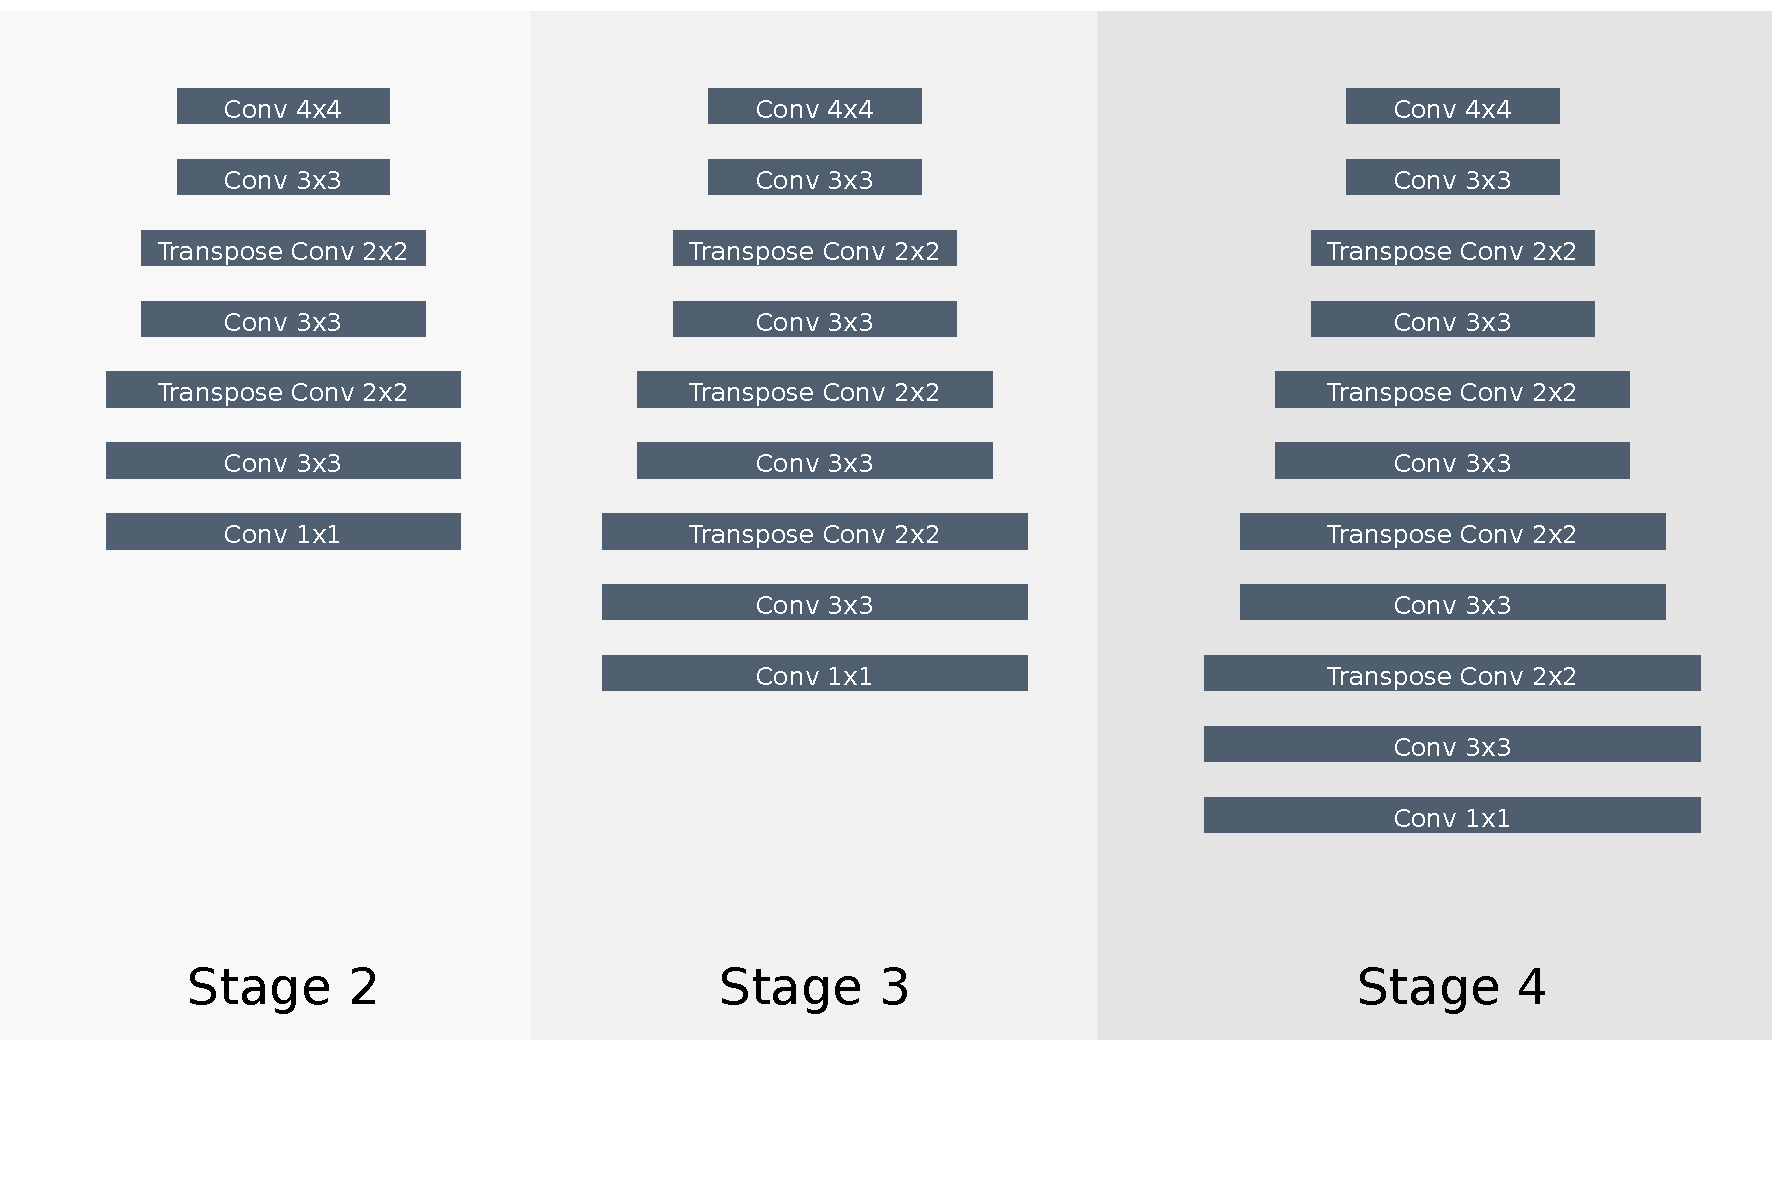
\includegraphics[width=\textwidth]{progressive_GAN_stages.pdf}
    \caption{Structure of the convolutions in the generator network for different stages of training in the progressive \acrshort{gan}.}
    \label{fig:prog_stages}
\end{figure}

\section{Progressive \acrshort{gan}}
The most advanced method tested in this project was the progressive \acrshort{gan}, proposed by \textcite{karras2017progressive}. The proposed advantages of this approach over other existing \acrshort{gan} variations is two-fold. Firstly, there is reason to believe that the quality and diversity of the generated samples are improved by the progressive training. Secondly, the training stability is believed to increase. However due to the novelty of the approach and the lack of extensive evaluations of different \acrshort{gans}, it is difficult to know for sure if this is the case.

The progressive \acrshort{gan} was adopted because of the proposed training stability that arises from progressivly increasing the complexity of the learned task. It was implemented using the default generator and discriminator. The training was divided in six stages, each stage producing images with four times the resoulution of the previous stage. As in the original article, each stage contained an extra 1x1 convolution to produce 2-channel images. The illustrated networks are therefore examples of stage-6 networks. To obtain a stage-5 network one should simply reshape the 1x1 convolutions and remove the two last (non 1x1) convolutions of the generator and the two first (non 1x1) convolutions of the generator. Figure \ref{fig:prog_stages} shows the structure of the generator network for different stages.

As in the original article, feature normalization, minibatch discrimination and smooth fade-in of new layers was implemented as closely as possible to the original formulation.


%\subsection{Freeze in new layers}
%\begin{figure}[t]
%    \centering
%    \begin{subfigure}[b]{0.45\textwidth}
%        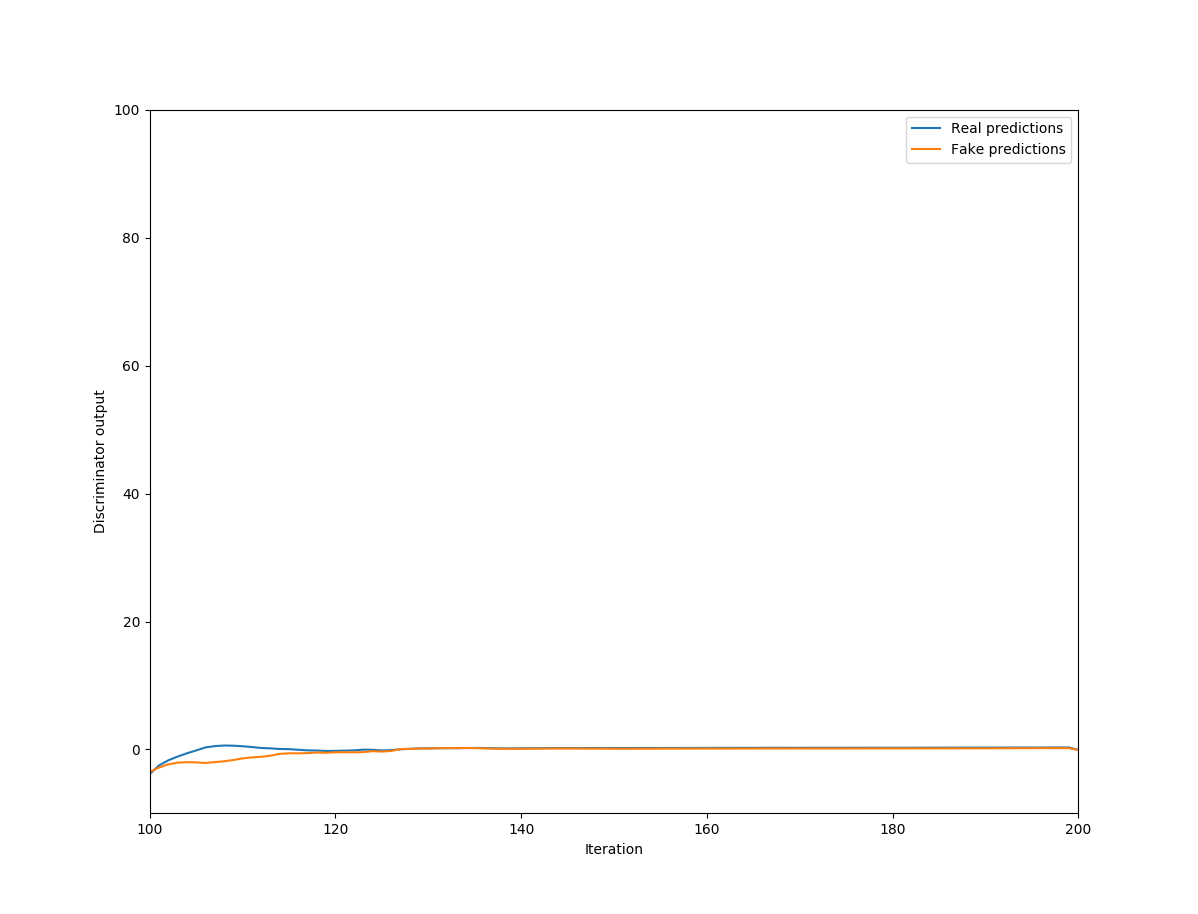
\includegraphics[width=\textwidth]{results/freezeInDG1.png}
%        \caption{Weight freezing in old layers}
%        \label{fig:freezeInDG1}
%    \end{subfigure}
%    \begin{subfigure}[b]{0.45\textwidth}
%        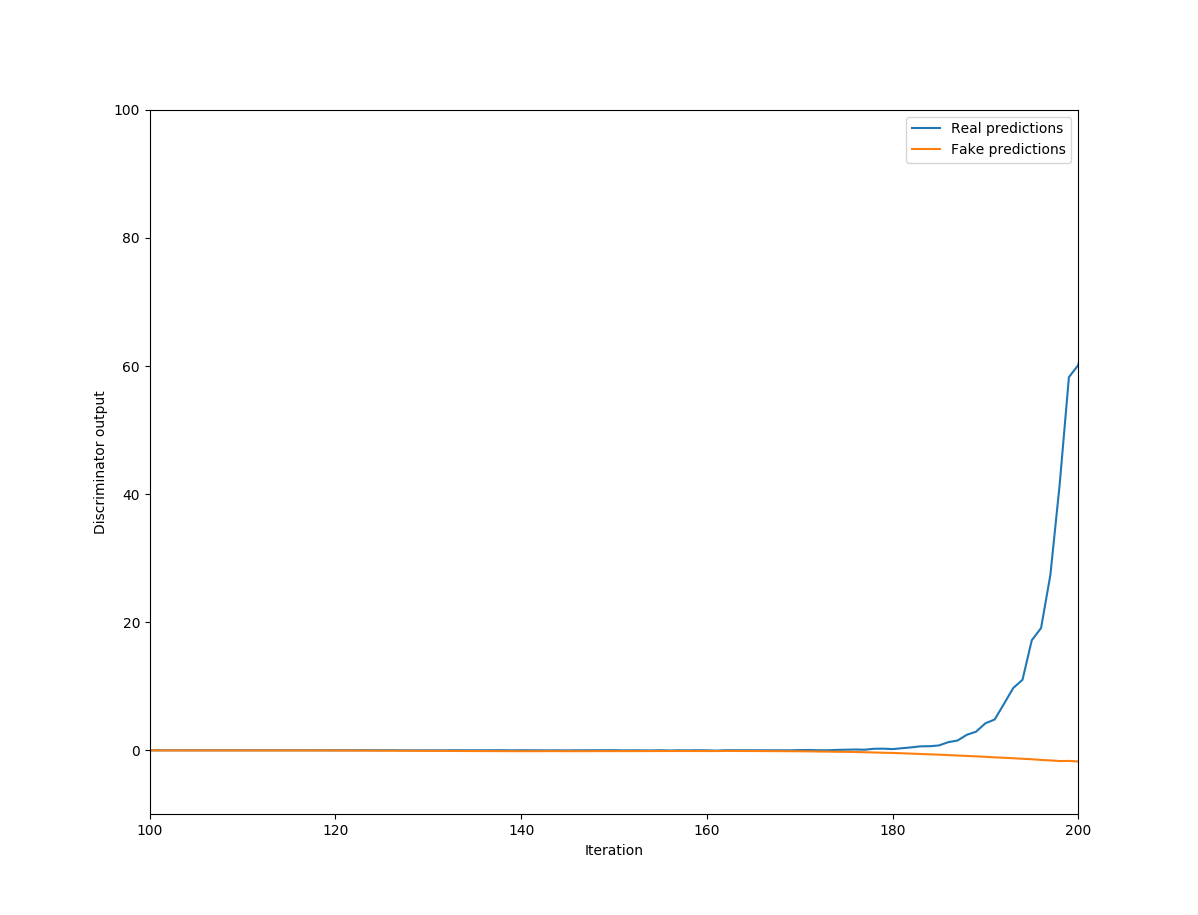
\includegraphics[width=\textwidth]{results/fadeInDG1.png}
%        \caption{Fade in new layers}
%        \label{fig:freezeInDG2}
%    \end{subfigure}
%    \caption{Discriminator output on real and fake images during transition between 16x16 and 32x32 resolution images for the different transition strategies.}
%    \label{fig:fadeVsFreeze}
%\end{figure}

\begin{figure}[t]
    \centering
    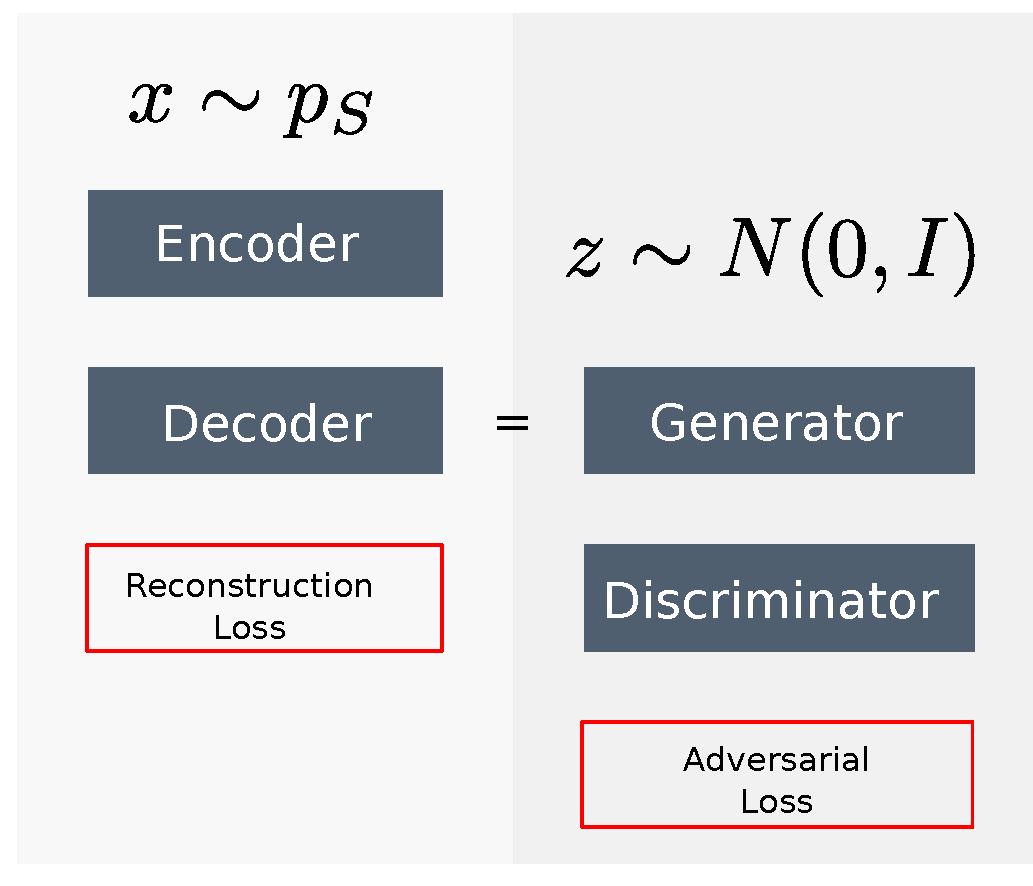
\includegraphics[width=0.7\textwidth]{aegan_illustration.pdf}
    \caption{The general structure of the neural networks in the \acrlong{aegan}. The left part of the image corresponds to an autoencoder and the right part corresponds to a \acrshort{gan}. The generator and decoder share the same architecture and parameters, otherwise the autoencoder training is completely decoupled from the \acrshort{gan} training.}
    \label{fig:aegan}
\end{figure}

\section{\acrlong{aegan}}
The final method tested in this project is based on a novel combination of autoencoders and \acrshort{gans}, named the \acrfull{aegan}. The proposed method consists of simultaneuously training a denoising autoencoder and a \acrshort{gan}, using the same network as generator and decoder. This is illustrated in figure \ref{fig:aegan}. The idea is conceptually similar to the \acrshort{vaegan} framework \parencite{LarsenSW15autoencodingbeyond}. There are two major differences between this method and the VAEGAN framework. First and foremost the autoencoder trained in this method is deterministic and trained with the mean squared error loss function. Secondly, the adversarial loss is not used to train the autoencoder, but instead a normal GAN is trained separately from the autoencoder but with the decoder network as the generator. 

Given enough capacity in the generator and encoder, the global minimum for the autoencoder training in this setting corresponds to the autoencoder learning the identity mapping. This causes the generator to generate realistic images on the points in the latent space the autoencoder maps the original data onto. The optimal generator in the \acrshort{gan} framework maps the entire latent space to realistic images. From this point of view the two objectives should lead to the same solution, however \acrshort{gans} tend to suffer from mode collapse and autoencoders often produce poor samples in terms of visual quality. Therefore if this method converges, it should force the decoded images to be sharp and the generator to capture the entire training data distribution. 
%\todocomment{I think that this paragraph is a bit wordy and is hard to follow. You could maybe improve it by adding a diagram to help illustrate the relationships between the encoder, decoder and GAN with respect to the latent space as well as contrasting it with VAEGAN. It is also worth stressing that this is a unique contribution if you haven't already done so already.}
% Idé till presentationen: "Variational autoencoders are stable and good at ...blablabla... . On the other hand there are two major problems with variational autoencoders, 1: they are variational (Åtgärda KL-term), 2: they are autoencoders (pixel-loss ersätts med GANs)."

\section{Training setup}
For the experiments, all models were trained using the Adamax optimizer \parencite{kingma2014adam} with $8$ samples per batch, a learning rate of $0.0001$, $\beta_1 = 0.5$ and $\beta_2 = 0.99$. The non-progressive models were trained for around $440$k iterations, however convergence of the methods might be either much faster or much slower than this depending on the model. The progressive training consisted of $100$k iterations per stage, with $10$k iterations of fade-in between the stages. 

